Lee con atención las siguientes situaciones y contesta lo que se te pide.

\begin{parts}
    % \begin{minipage}[t]{0.4\textwidth}
    %     \begin{figure}[H]
    %         \raggedright
    %         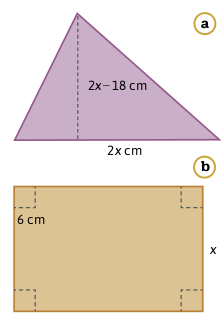
\includegraphics[width=0.9\linewidth]{../images/figuras2.7.png}
    %         \captionof{figure}{(a) Triángulo, (b) Pieza rectangular para armar una caja.}
    %         \label{fig:figuras2.7}
    %     \end{figure}
    % \end{minipage}\hfill
    % \begin{minipage}[t]{0.5\textwidth}
    %     \part El triángulo de la figura \ref{fig:figuras2.7}a tiene área igual a 52 cm$^2$, encuentra las medidas de su base y de su altura.

    %     \begin{solutionbox}{3.5cm}

    %     \end{solutionbox}

    %     \part Una pieza rectangular como la de la figura \ref{fig:figuras2.7}b es 4 cm más larga que ancha. Con ella se construye una caja de 840 cm$^3$ cortando un cuadrado
    %     en cada esquina y doblando los bordes. Escribe las medidas de la altura y el volumen de la caja, así como los lados de la pieza rectangular.
    %     \begin{solutionbox}{3.5cm}

    %     \end{solutionbox}
    % \end{minipage}

    \part El área de un rectángulo es 28 cm$^2$. Tiene 3 cm más de largo que de ancho. ¿Cuáles son sus dimensiones?

    \begin{solutionbox}{9cm}

    \end{solutionbox}

    \part Un terreno rectangular tiene área de 750 m$^2$. Se coloca una cerca alrededor de los 110 m de perímetro. Calcula las dimensiones del terreno.

    \begin{solutionbox}{9cm}

    \end{solutionbox}

    % \part Un rectángulo tiene el ancho más corto que el largo por 3 cm. El área de la figura es de 51 cm$^2$. ¿Qué medidas tiene?

    % \begin{solutionbox}{3cm}

    % \end{solutionbox}
\end{parts}